\section{Kailath 4.3-4}
The state-space model of the inertial navigator is 
\begin{align*}
    \begin{pmatrix}
        \dot v \\ \dot \varphi \\ \dot \varepsilon
    \end{pmatrix} &= \begin{pmatrix}
        0 & -1 & 0 \\ 1 & 0 & 1 \\ 0 & 0 & 0
    \end{pmatrix}\,\begin{pmatrix}
        v \\ \varphi \\ \varepsilon
    \end{pmatrix} + \begin{pmatrix}
        0 \\ 0 \\ w
    \end{pmatrix}
\end{align*}
(a) Determining the solutions. 
\begin{align*}
    X(s) = 0 \quad \det{\left(sI - A\right)} &= 0 \\
    \det\begin{pmatrix}
        s & 1 & 0 \\ -1 & s & -1 \\ 0 & 0 & s
    \end{pmatrix} &= 0\\
    s\,\left(s^2 + 1\right) &= 0.
\end{align*}
The open-loop eigen values are $\lambda_1 = 0$, $\lambda_{2,3} = \pm j$

(b) observer design 
\begin{align*}
    y = \begin{pmatrix}
        1 & 0 & 0
    \end{pmatrix}\,\begin{pmatrix}
        v \\ \varphi \\ \varepsilon 
    \end{pmatrix}
\end{align*}
The observer is 
\begin{align*}
    \dot{\hat X} &= A\,\hat X + B\,u + K\,\left(y - C\,\hat X\right) \\
    \begin{pmatrix}
        \dot{\hat v} \\ \dot{\hat \varphi} \\ \dot{\hat \varepsilon}
    \end{pmatrix} &= \begin{pmatrix}
        0 & -1 & 0 \\ 1 & 0 & 1 \\ 0 & 0 & 0
    \end{pmatrix}\,\begin{pmatrix}
        \hat v \\ \hat \varphi \\ \hat \varepsilon
    \end{pmatrix} + \begin{pmatrix}
        0 \\ 0 \\ w
    \end{pmatrix} + K\,\left(y - \begin{pmatrix}
        1 & 0 & 0
    \end{pmatrix}\,\begin{pmatrix}
        \hat v \\ \hat \varphi \\ \hat \varepsilon
    \end{pmatrix}\right)
\end{align*}
The closed-loop observer poles 
\begin{align*}
    \alpha_\mathcal{O}(s) &= \text{det}\left(SI - A + K\,C\right) \\
    &=  \det\left(\begin{pmatrix}
        s & 0 & 0 \\ 0 & s & 0 \\ 0 & 0 & s
    \end{pmatrix} - \begin{pmatrix}
        0 & -1 & 0 \\ 1 & 0 & 1 \\ 0 & 0 & 0
    \end{pmatrix} + \begin{pmatrix}
        k_1 \\ k_2 \\ k_3 
    \end{pmatrix}\,\begin{pmatrix}
        1 & 0 & 0
    \end{pmatrix}\right)\\
    &= \det\begin{pmatrix}
        k_1 + s & 1 & 0 \\ k_2 - 1 &  s -1 \\ k_3 & 0 & s
    \end{pmatrix} \\
    &= s^3 + k_1\,s^2 + \left(1 - k_2\right)\,s - k_3
\end{align*}
The closed-loop observer poles are $s = -10$, $s = -0.1$, $s = -0.1$
\begin{align*}
    \alpha_\mathcal{O}(s) &= \left(s + 10\right)\,\left(s + 0.1\right)\,\left(s + 0.1\right) \\
    &= s^3 + 10.2\,s^2 + 2.01\,s + 0.1
\end{align*}
The gains are 
\begin{align*}
    K = \begin{pmatrix}
        k_1 & k_2 & k_3
    \end{pmatrix}^T = \begin{pmatrix}
        10.2 & -1.01 & -0.1
    \end{pmatrix}^T
\end{align*}
The simulation results of the observer is shown in the next page
\clearpage

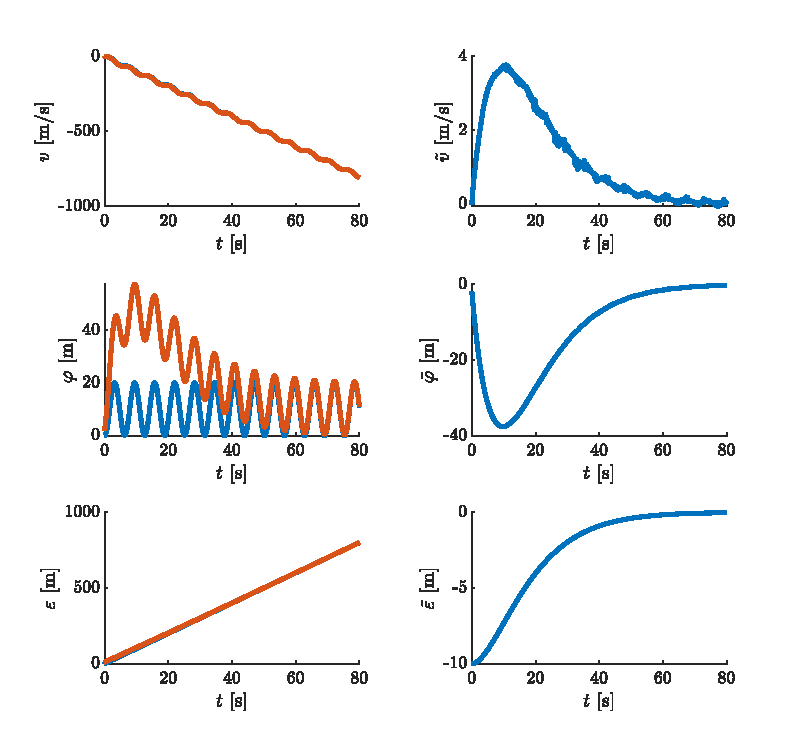
\includegraphics{figures/le4_3_7a.pdf}

The estimated states from the observer are shown in orange and the 'true' states are shown in blue.

(c) The \emph{second order} observer. 
Original state equations
\begin{align*}
    \begin{pmatrix}
        \dot v \\ \dot \varphi \\ \dot \varepsilon
    \end{pmatrix} &= \begin{pmatrix}
        0 & -1 & 0 \\ 1 & 0 & 1 \\ 0 & 0 & 0
    \end{pmatrix}\,\begin{pmatrix}
        v \\ \varphi \\ \varepsilon
    \end{pmatrix} + \begin{pmatrix}
        0 \\ 0 \\ w
    \end{pmatrix}, &  
    \text{or } \begin{pmatrix}
        \dot \varepsilon \\ \dot \varphi \\ \dot v 
    \end{pmatrix} &= \begin{pmatrix}
        0 & 0 & 0 \\ 1 & 0 & 1 \\ 0 & -1 & 0
    \end{pmatrix}\,\begin{pmatrix}
        \varepsilon \\ \varphi \\ v
    \end{pmatrix} + \begin{pmatrix}
        w \\ 0 \\ 0
    \end{pmatrix}
\end{align*}
Considering partitioned state equations 
\begin{align*}
    \begin{pmatrix}
        \dot x_r \\ \dot x_n 
    \end{pmatrix} &= \begin{pmatrix}
        A_r & a_r \\ a_n & a_{nn} 
    \end{pmatrix}\,\begin{pmatrix}
        x_r \\ x_n 
    \end{pmatrix} + \begin{pmatrix}
        b_r \\ b_n 
    \end{pmatrix}\,u(t) & y &= x_n \\
    \begin{pmatrix}
        \begin{pmatrix} \dot{\hat \varepsilon} \\ \dot{\hat \varphi} \end{pmatrix} \\ \dot{\hat v} 
    \end{pmatrix} &= \begin{pmatrix}
        \begin{pmatrix}
            0 & 0 \\ 1 & 0
        \end{pmatrix} & \begin{pmatrix}
            0 \\ 1
        \end{pmatrix} \\
        \begin{pmatrix}
            0 & -1
        \end{pmatrix} & 0
    \end{pmatrix}\,\begin{pmatrix}
        \begin{pmatrix} \hat \varepsilon \\ \hat \varphi \end{pmatrix} \\ \hat v
    \end{pmatrix} + \begin{pmatrix}
        \begin{pmatrix} w \\ 0 \end{pmatrix} \\ 0
    \end{pmatrix} & y &= v
\end{align*} 

\fbox{\parbox{0.95\textwidth}{
    Change in partitioning affects the pole placement of the reduced order observer, with $\begin{pmatrix}
        \begin{pmatrix}
            \varphi & \varepsilon
        \end{pmatrix} & v
    \end{pmatrix}^T$, only one pole (of the reduced order observer) can be placed arbitrarily.
}}

The closed-loop poles 
\begin{align*}
    \alpha_\mathcal{O}(s) &= \det\left(sI - A_r + L\,a_n\right) \\
    &= \det\left(\begin{pmatrix}
        s & 0 \\ 0 & s
    \end{pmatrix} - \begin{pmatrix} 0 & 0 \\ 1 & 0 \end{pmatrix} + \begin{pmatrix}
        l_1 \\ l_2
    \end{pmatrix}\,\begin{pmatrix} 0 & -1 \end{pmatrix}\right) \\
    &= \det\left(\begin{pmatrix}
        s-1 & -l_1 \\ -1 & s-l_2
    \end{pmatrix}\right) = s^2 -l_2\,s - l_1
\end{align*}

The closed-loop observer poles are $s = -0.1$, $s = -0.1$
\begin{align*}
    \alpha_\mathcal{O}(s) &= \left(s + 0.1\right)\,\left(s + 0.1\right) = s^2 + 0.2\,s + 0.01
\end{align*}

The gains are 
\begin{align*}
    L = \begin{pmatrix}
        l_1 & l_2 
    \end{pmatrix}^T = \begin{pmatrix}
        -0.01 & -0.2
    \end{pmatrix}^T
\end{align*}

The observer is designed as, 
\begin{align*}
    \dot{\hat \theta} &= \left(A_r - L\,a_n\right)\,\theta + \left(a_r - L\,a_{nn} + A_r\,L - L\,a_n\,L\right)\,y + (b_r - b_n)\,u \\
    \hat x_r &= \theta + L\,y \\
    \hat x_n &= x_n = y
\end{align*}
% The closed-loop poles (altered partioning)
% \begin{align*}
%     \alpha_\mathcal{O}(s) &= \det\left(sI - A_r + L\,a_n\right) \\
%     &= \det\left(\begin{pmatrix}
%         s & 0 \\ 0 & s
%     \end{pmatrix} - \begin{pmatrix} 1 & 0 \\ 0 & 0 \end{pmatrix} + \begin{pmatrix}
%         l_1 \\ l_2
%     \end{pmatrix}\,\begin{pmatrix} 0 & -1 \end{pmatrix}\right) \\
%     &= \det\left(\begin{pmatrix}
%         s-1 & -l_1 \\ 0 & s-l_2
%     \end{pmatrix}\right) = \left(s - 1\right)\,\left(s - l_2\right)
% \end{align*}
% Placing the estimator poles at $-0.1$, gives $l_2 = -0.1$.

The simulation results of the observer are shown below, where the estimated states from the observer are shown in orange, and the 'true' states are shown in blue.

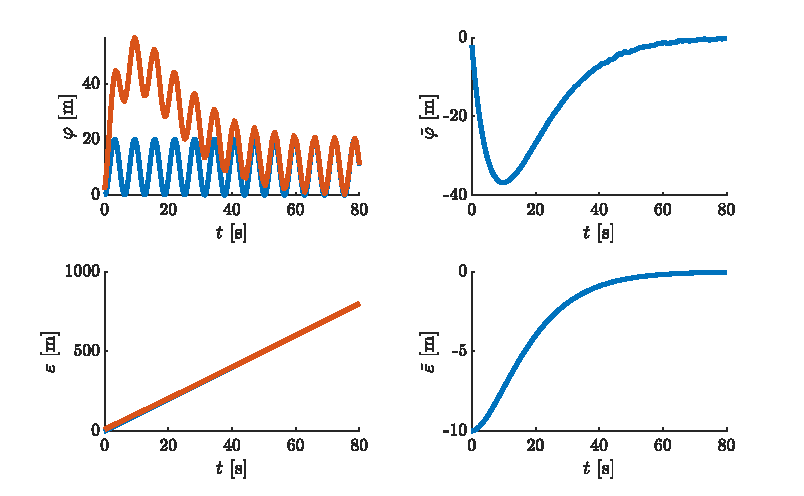
\includegraphics{figures/le4_3_7b.pdf}

\fbox{\parbox{0.95\textwidth}{
    The reduced-order and the full-order observer are similar in performance.
}}

\section*{Code}
\matlabheading{simulation (true system)}

\begin{matlabcode}
clear;
u = 10;
A = [0 -1 0; 1 0 1; 0 0 0];
B = [0; 0; 1]; C = [1 0 0];
int_nav = @(t,x) A*x + B*u;

% simulation
y0 = [0; 0; 0]; % initial states
tspan = [0 80]; % [s]
[t, y] = ode45(@(t,y) int_nav(t,y),tspan,y0);
\end{matlabcode}


\matlabheading{Observer simulation}

\begin{matlabcode}
% state observer 
K = [10.2; -1.01; -0.1];
mesh = @(x) interp1(t,y(:,1),x,'spline');
obs_int_nav = @(t,x) A*x + B*u + K*(mesh(t) - C*x);

% simulation 
y0 = [0; 2; 10]; % initial states
[to, yo] = ode45(@(t,y) obs_int_nav(t,y),tspan,y0); 

% error
for ii = 1:width(y)
    yq = interp1(t,y(:,ii),to);
    eq(:,ii) = yq - yo(:,ii);
end
\end{matlabcode}


\matlabheading{Reduced order observer simulation}

\begin{matlabcode}
% A-matrix partition
Ar = [0 0; 1 0];
cr = [0 -1];
br = [0; 1];
ann = 0;
% B_matrix
gr = [1; 0];
gn = 0;
% observer gain
L = [-0.01; -0.2];
% state observer
red_obs_int_nav = @(t,z) (Ar - L*cr)*z ... 
                  + (br -L*ann + Ar*L - L*cr*L)*mesh(t) ...
                  + (gr - L*gn)*u;

% simulation
y0 = [10; 2]; % initial states
[tr, zo] = ode45(@(t,y) red_obs_int_nav(t,y),tspan,y0); 

% states
for ii = 1:length(tr)
    xr(ii,:) = zo(ii,:) + (L*mesh(tr(ii)))';
end

% error
yq = interp1(t,y(:,3),tr);
eq2(:,1) = yq - xr(:,1);
yq = interp1(t,y(:,2),tr);
eq2(:,2) = yq - xr(:,2);
\end{matlabcode}